\documentclass[../main.tex]{subfiles}
\usepackage[english]{babel}
\graphicspath{{\subfix{../images}}}
\begin{document}

\section{Digital images}
Images are now belief to play a key role in the diagnosis procedure and, overall, in the medical field. When it comes to visual diagnosis of a patient all information needed by the medical doctors can be stored in a digital representation thanks to digital images. 
The advantages in using digital images are numerous: they are immediately available and they can be stored easily with a consistent image quality, their post-processing is handable with computers and they allow digital watermarking to prove copyright ownership \cite{journal_of_dermatology}.  

Some crucial information and markers are detected by clinical experts during images' evaluation. Taking into consideration that clinical imaging departments could produce even hundreds of thousands of images per year, it is fundamental to understand the information carried by these and to be able to extract such information \cite{info_in_images}.

\subsection{Definition of digital images}\label{sec:definition-of-images}

Digital images could be easily defined as a discrete numerical representation of an object. In order to understand how a complex object could be represented by a set of numbers one has to understand what are the processes involved in the image formation and how it is stored as mere numbers.
The real phenomenon which undergoes the digital image formation happens in the digital camera, where the light reflected by the object is focused onto a grid of photosensors which acquire the light intensity and record it as an array of picture elements (\textit{pixels}) \cite{bourne2010fundamentals}.

\begin{figure}[H] 
\begin{center}
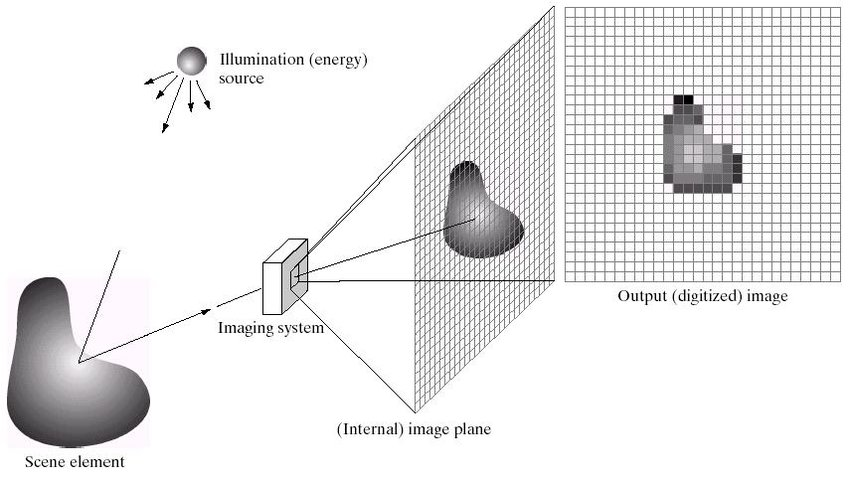
\includegraphics[width=11cm]{images/Image-Acquisition-Model.png}
\caption{\small{Representation of the image acquisition process: the light is reflected from the object, then it passes through the imaging system. The intensity is absorbed by photosensors that convert the electromagnetic signal into a grid of pixels which forms the output image.\cite{CNN_chapter13}}}\label{fig:Image_acquisition}
\end{center}
\end{figure}

The general aim of the digital image acquisition is to transform the continuous light signal into a discrete array of numbers (usually integers) which can be processed by computers \cite{image_acquisition_article}. This procedure , as shown in Figure \ref{fig:Image_acquisition}, is characterized by several components which have a contribution on the output images:

\begin{itemize}
    \item light intensity reflected from the object;
    \item acquisition device;
    \item number of grid elements;
    \item intensity displayed by each grid element.
\end{itemize}

These elements participate in different steps of the image formation. The light intensity and the acquisition device play a role during the acquisition procedure; whereas, the number of grid elements and the intensity displayed are responsible for the resolution of the digital image.

\subsubsection{Acquisition distortions}

The signal incoming from the object can be modelled as a continuous function of the spatial coordinates of the object's space $g(s,t)$, defining the output image as a function of the coordinates in the image plane $f(x,y)$, we can find a relation between them which could be seen as:

\begin{equation} \label{eq:imageacquisition}
    f(x,y) = \int_{-\infty}^{+\infty} h(x,y,s,t)g(s,t) dsdt
\end{equation}

where $h(x,y,s,t)$ is the response of the acquisition system which describes how much each $(s,t)$ point in the object space contributes to the image point $(x,y)$.

Unfortunately, the resulting image could suffer for uncertainties and fluctuations during the signal's recording. This phenomenon could have many sources (electronic components, interference ...) and it is described as \textit{noise}.
To be more precise one should add another term to the Equation \ref{eq:imageacquisition} and so the equation will be:

\begin{equation} \label{eq:imageacquisition+noise}
    f(x,y) = \int_{-\infty}^{+\infty} h(x,y,s,t)g(s,t) dsdt  + n(x,y)
\end{equation}

where the additive component $n(x,y)$ is a way to introduce the noise into the function. 
In many situation the noise $n(x,y)$ could be modelled as a Gaussian function.

A method to measure these inevitable spatial distortions is to display the \textit{Point Spread Function} (PSF) which is a function that describes which size and shape an infinitesimal point in the $(s,t)$ space would have in the $(x,y)$ image space \cite{bourne2010fundamentals}.

\subsubsection{Matrix representation}\label{sec:matrix_representation}

The distortions explained in the previous section remains still valid, but, for sake of simplicity, we assume that it is possible to acquire a perfect continuous signal.

From a mathematical standpoint we can see the digital image as a quantization of a  function of two spatial continuous dimensions $g(s,t)$ which represents the continuous signal coming from the light reflected from the object.
Thanks to the photosensors this continuous signal is sampled and into a 2-D array containing $M$ rows and $N$ columns. Therefore, the digital image could be represented as a function $f(x,y)$ where $(x,y)$ are discrete spatial coordinates which compose the spatial domain of the image \cite{digital_image_processing_gonzales}:

\begin{equation}\label{eq:image_matrix}
    f(x,y) = \begin{bmatrix} f(0,0) & f(0,1) & \dots & f(0,N-1)\\
                            f(1,0) & f(1,1) & \dots & f(1,N-1)\\
                            \vdots & \vdots &     & \vdots \\
                            f(M-1,0) & f(M-1,1) & \dots & f(M-1,N-1)
             \end{bmatrix}
\end{equation}

Each element $f(i,j)$ of the matrix of the Equation \ref{eq:image_matrix} represents an image element or pixel. The partition of the $(s,t)$ space into a grid can be defined as \textit{sampling process} \cite{digital_image_processing_gonzales}. Rows and columns are responsible for the spatial location in the image and the corresponding value represents the intensity in that specific point, i.e. it represents the grey level  in black and white images\cite{annadurai2007fundamentals}. The functional assignment of an intensity value to each point $(x,y)$ is called \textit{quantization}\cite{digital_image_processing_gonzales}.
To define the values for each pair of coordinates an integer value is usually chosen among the powers of 2:

\begin{equation}\label{equation_intensity_levels}
    I = 2^{k}
\end{equation}

The discrete value for the intensity $I$ at each image point is an integer ranging in the interval $[0,2^{k}-1]$. 
In this way the dynamic range of the image, a quantity which describes the ratio between the highest and lowest value of I \cite{dynamic_range}, is defined by the $k$ parameter. If we consider a binary image, $k=1$ since there are only $2^{1}=2$ possible levels of intensity (0 or 1). On the other hand, for grey scale images $k$ is usually 8. As a consequence, the total image would present $2^{8}=256$ grey levels with values in $[0,255]$.

\subsubsection{Gray-level histogram}

Starting from the matrix representation of the digital images, it is possible to count the occurrences of each grey-level value in the full image to produce a grey-level histogram \cite{fiete2010modeling}.  

Following the same formalism and considering an $M\times N$ image with a intensity level range of $[0, I-1]$, the grey-level histogram represents the discrete function:
\begin{equation}
    h(i_{j})=n_{j} 
\end{equation}

where $i_{j}$ is one of the image grey-level values and $n_{i}$ is the sum of pixels with intensity $i_{j}$.

The histogram loses all the spatial information of the image, but, if it is normalized by the total number of pixels $M\times N$, it represents the statistical distribution of the grey-levels. 

Looking at the Figure \ref{fig:histo}, it is possible to understand which information is embedded in the grey-level histogram. For dark images the distribution is shifted towards low values; on the contrary,bright scenes show a considerable concentration on the right side of the x-axis (higher values). Moreover, the image contrast can be associated with the spread of the distribution along all the intensities.

\begin{figure}[H] 
\begin{center}
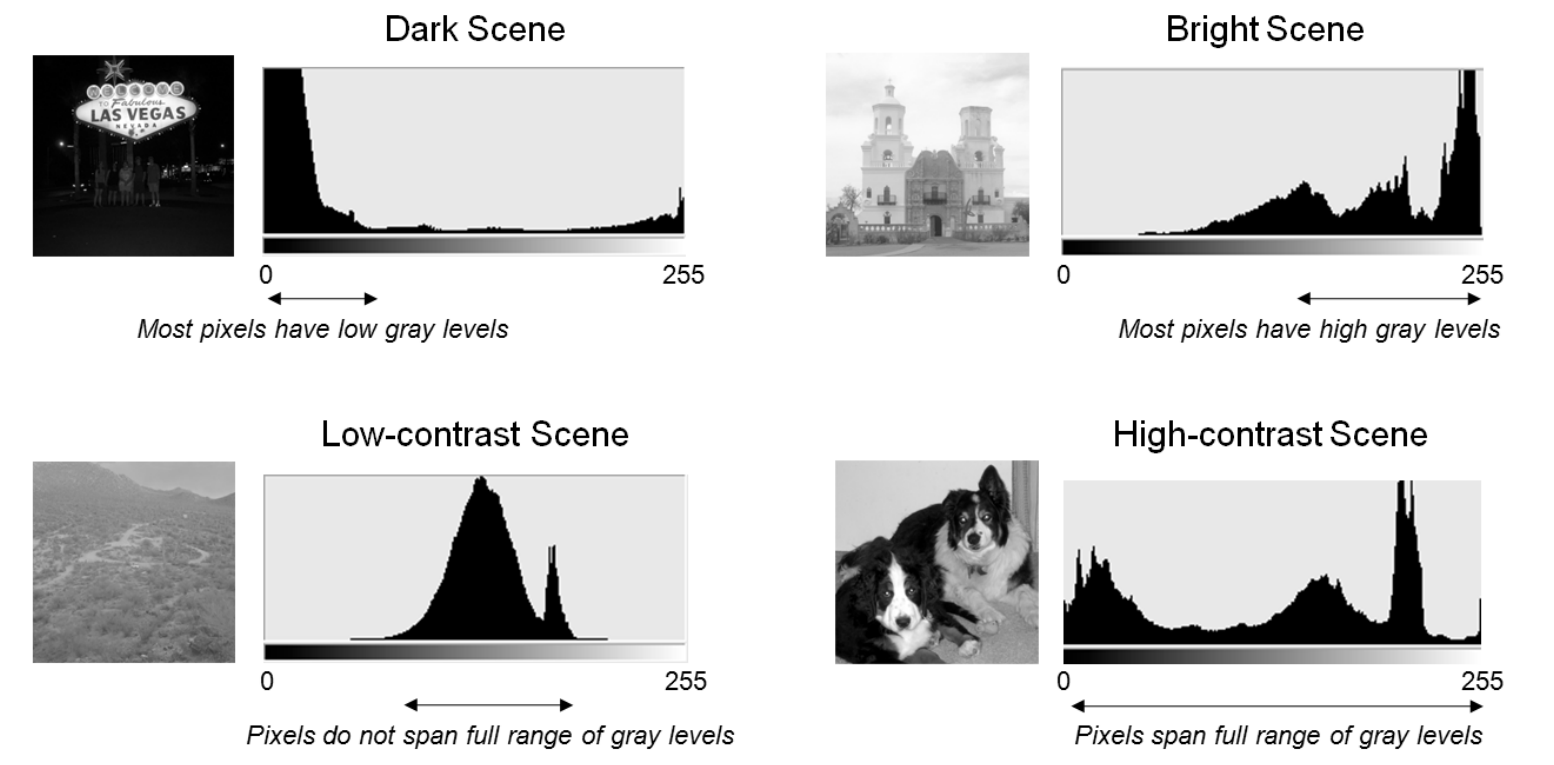
\includegraphics[ height= 8.3cm]{images/image_histogram.png}
\caption{\small{Representation, taken from \cite{fiete2010modeling}, of four images with their respective grey-level histograms.}}\label{fig:histo}
\end{center}
\end{figure}

This approach becomes useful when the analysis focuses  on image brightness and contrast, without needing any spatial information, i.e. contrast enhancement, brightness enhancement, thresholding.


\subsubsection{Spatial resolution and dynamic range}

Given the matrix formulation of Equation \ref{eq:image_matrix}, one could easily understand the importance of the choice of grid elements' number and dimensions as well as the number of discrete levels for the intensity representation.

The number of pixels of an image determines the spatial quality of the overall outcome, the procedure to select the appropriate amount of them is to follow the Nyquist–Shannon sampling theorem \cite{Shannon1949}. It sets a lower bound for the spatial sampling rate which must be twice smaller than the smallest detail of the image and this it is possible to avoid artifact due to incorrect sampling.

The number and dimensions of pixels define the \textbf{spatial resolution} of the image which describes the smallest detail which can be observed in an image \cite{digital_image_processing_gonzales}. The most used measure for the spatial resolution are \textit{dpi} i.e dots per inch. The reference with the spatial unit is helpful in order to better describe the image quality rather than using solely pixels.
A 300 dpi image is considered to be an high resolution picture for printing. \textit{Bittorf et al.} \cite{resolution_requirements} had indeed showed that there is a critical resolution of 512 dpi for the human eye. Below this number two images with different dpi are promptly recognize to be of different quality. Even if the critical number depends on several conditions (purpose, subject, output device etc.), this study shows that producing images with enormous value of dpi does not necessary improve the perceived quality, but it certainly does with storage requirements.
 
As for the spatial resolution, the \textbf{dynamic range} or intensity resolution can be defined as the smallest change in the intensity level that can be perceived\cite{digital_image_processing_gonzales}. The intensity levels defined in the Equation \ref{equation_intensity_levels} are a good measure of dynamic range. They are usually expressed in the number of bits used to express the levels (the $k$ parameter in Equation \ref{equation_intensity_levels}). 

A good dynamic range avoids artifacts and distortions of the brightness representation. High intensity resolution leads to higher visibility in low contrast images but could be worsen by statistical noise.

\subsection{Color Images}\label{sec:color-images}

The matrix definition of images showed in Section \ref{sec:matrix_representation} explains how each grid element is able to reproduce a discrete level of the intensity registered by the acquisition device. However, the one dimensional representation does not take into account the possibility of a colored image.
To model different combinations of color it is helpful to recall the \textit{trichromacy} theory \cite{young}. Together with further experimental studies, it proved that the human visual system is built such that every possible perceived color can be decomposed in a combination of three primaries. In fact, the light is focused onto the retina in the human eye, then three types of cones (color sensors present inside the retina) absorb different wavelength of visible light.

Defining $f(\lambda)$ the continuous spectral distribution incident on the retina as a function of $\lambda$ the wavelength the responses of cones were modelled in \cite{colors-images} as:

\begin{equation}
   c_{i} = \int_{}^{} s_{i}(\lambda)f(\lambda)d\lambda   \qquad i=1,2,3
\end{equation}

where $s_{i}(\lambda)$ describes the $i$th cone's sensitivity. Typically the wavelength range for which there are non-zero sensitivities is $[360 nm, 830 nm]$.



Following the principles of such theory, some mathematical models were developed to describe colors as a combination of three independent variables, accounting contributions that dates back to Grassmann \cite{grassmann1854theory} and Maxwell \cite{maxwell1856theory}.

Several color coordinate systems were defined in order to model the \textit{trichromacy}. A complete list of them is available in \cite{jain1989fundamentals}. The principal ones are:

\begin{description}
    \item[RGB]: a combination of monochromatic primaries corresponding to red(R) = 700nm,
    green(G) = 546.1 nm and blue 435.8 nm. It is widely used in modern digital images
    \item[CMY]: secondary colors like cyan(C), magenta(M) and yellow(Y) are used as base. The conversion from \textit{CMY} to \textit{RGB} is: 
    
    \begin{center}
    \begin{math}
    \begin{bmatrix}
    C \\ M \\ Y
    \end{bmatrix} = \begin{bmatrix}
    1 \\ 1 \\ 1
    \end{bmatrix} - 
    \begin{bmatrix}
    R \\ G \\ B
    \end{bmatrix}
    \end{math}
    \end{center}
    
    assuming the values normalized to 1.
    \item[HSV]: this model does not take in consideration pure colors. It uses hue(H), saturation(S) and value(V) to describe the possible combinations. Respectively, the three values represent the dominant color, its purity and its brightness on grey scale.
    \item[Lab]: which combines \textit{RGB} and \textit{HSV} taking as variables the brightness(L), red-green contents(a) and yellow-blue contents(b)
\end{description}

Focusing on the most common \textit{RGB} system,  we can think to this model based on Cartesians coordinates where each point in the  \textit{RGB} space can be represented as a combination of the primaries. Assuming the values normalize to 1 we can model some common colors:

\begin{center}
\begin{tabular}{ c c c }
 red=(1,0,0) & green=(0,1,0) & blue=(0,0,1) \\ 
 black==(0,0,0) & white=(1,1,1) & grey=(0.5,0.5,0.5) \\  
 cyan=(0,1,1) & magenta=(1,0,1) & yellow=(1,1,0)    
\end{tabular}
\end{center}

as we can see the previous conversion from \textit{CMY} to \textit{RGB} is consistent with this definition.

The \textit{RGB} model is compatible with the matrix formalism used to describe pixels of digital images. However, if for grey scale images the single matrix is enough to represent the grey level intensity, in the \textit{RGB} model we need to explore the third dimension. The matrix become a tri-dimensional tensor showed in Figure \ref{fig:rgb}.

\begin{figure}[H] 
\begin{center}
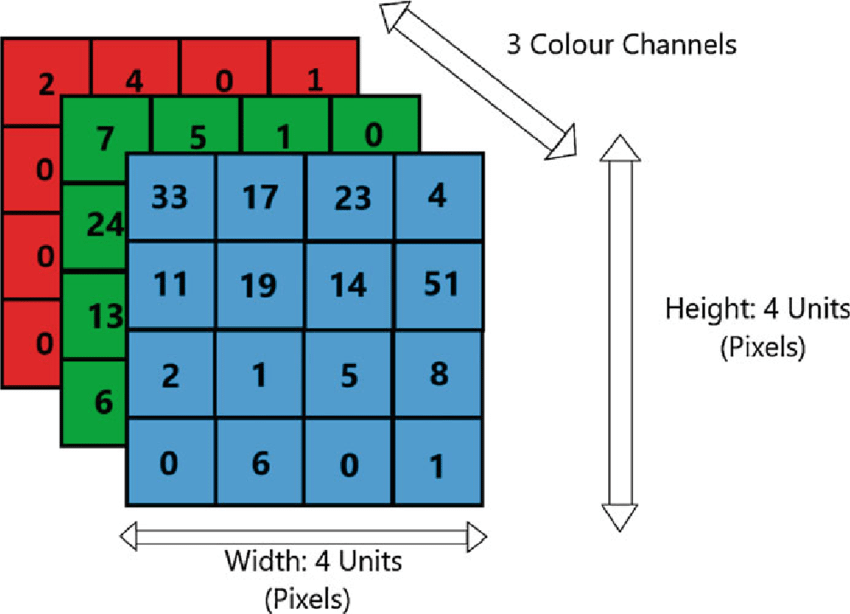
\includegraphics[width=11cm]{images/rgb.png}
\caption{\small{Representation of the RGB-image matrix. The colors channels show the same dimension but different intensity values. The final color for each pixel is given by the combination of the three.}}\label{fig:rgb}
\end{center}
\end{figure}

The Height and Width still describe the spatial information of the image. Whereas, the Color dimension is divided into three channels, each one of them is responsible for the representation of the color intensity of one of the primaries, the resulting digital image is simply the superposition of the three color channels.




\subsection{Image formats}

Digital images can be stored in different formats, they are suitable for particular data type and usage.  In \cite{bourne2010fundamentals} Bourne states that choosing a specific format affects:
\begin{itemize}
    \item the size of the image;
    \item the amount of metadata (information on acquisition device and procedures) storable;
    \item the integrity of the data;
    \item the image transmission.
\end{itemize}

In several cases the images are stored in formats which benefit of compression. Compression is a method to ease image storaging and transmission, but it can cause information loss. The different compression formats are divided into two categories \cite{digital_processing_matlab}:
on one hand, if the image can be fully reconstructed from the compressed data without loosing information, we are exploiting \textit{lossless compression}; on the other hand, if the redundant information is removed from the image, we are in the case of \textit{lossy compression}.
Both of these compression formats are useful to shrink the storage volume, but in the case of \textit{lossy compression} some data are irreparably lost, with consequent possible problems during image analysis.

Data type is another fundamental variable to take into consideration when choosing a file format. As mentioned in Section \ref{sec:definition-of-images} integer numbers are the most used quantity to describe pixels' intensity, but other data types are also used in digital imaging. 

\textit{Binary}, \textit{Grey-scale} and \textit{Color} images make use of the integer definition of Equation \ref{eq:image_matrix}.
\begin{itemize}
    \item \textit{Binary} images are  characterized by $k=1$, so they are able to show only black and white pixels. This data type is widely used for images where some objects or foreground have to be separated from the background, i.e. image segmentation's masks;
    \item \textit{Grey-scale} images are usually represented with 8-bit depth ($k=8$), at each pixel value is associated a grey level intensity ranging from 0=black up to 255=white;
    \item \textit{Color} images were already explained in Section \ref{sec:color-images}, they generally exploit integer tensors of three color channels which depend on the chosen color model.
\end{itemize}

\textit{Floating-point} images store different type of data. The floating-point numbers used in this kind of images are basically Real numbers organized in the same matrix form. Such images are useful to represent precise measurements and are defined in a range which depends on the number of image's bits.

Some of the most important images' formats are represented in Figure \ref{fig:table_formats}.

\begin{figure}[H] 
\begin{center}
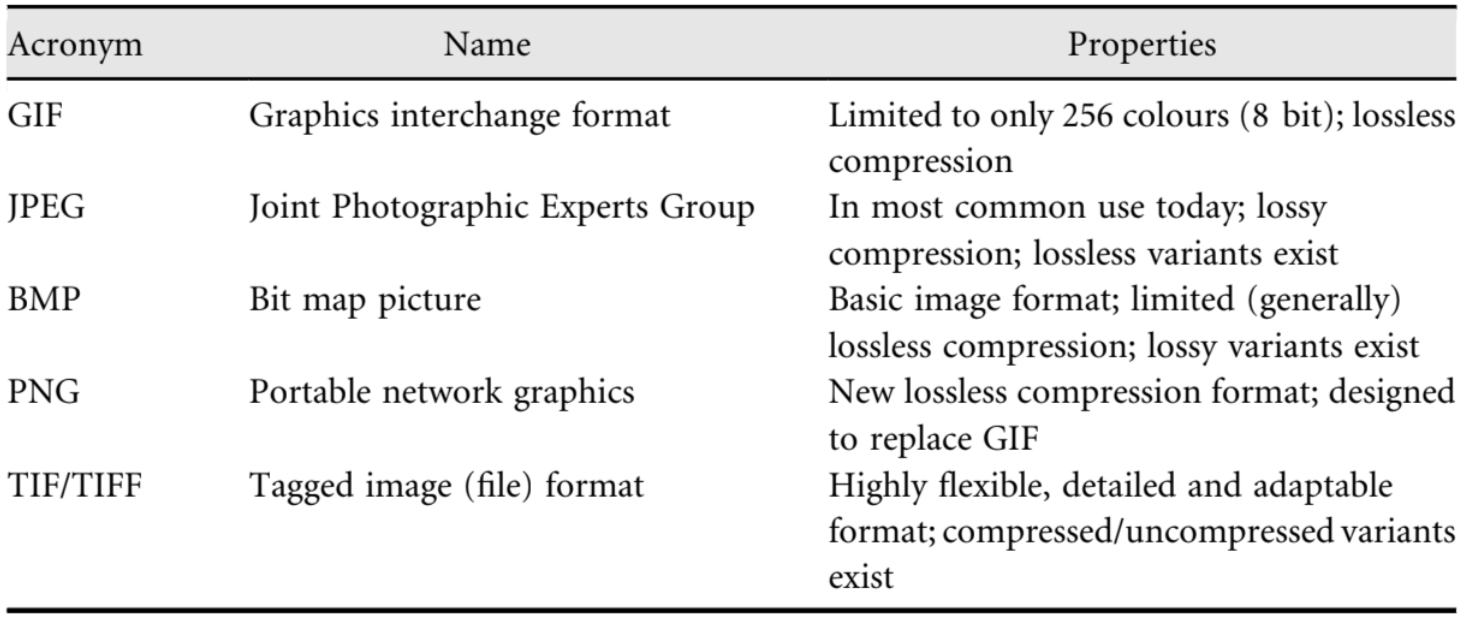
\includegraphics[width=11cm]{images/image_formats.png}
\caption{\small{Most used images' formats with their compression properties, from \cite{digital_processing_matlab}}}\label{fig:table_formats}
\end{center}
\end{figure}

JPG is the most used for digital cameras and smartphones thanks to the huge reduction on image storaging, it can store 24-bit RGB color images but its lossy compression does not suite well for image processing applications. By contrast, the PNG format is the most used in digital imaging analysis due to his lossless compression. It  also overcomes the problem with the GIF format (capable of storing only 256 colors) allowing two storage systems of 24/48 bits per pixel\cite{roelofs1999png}, such bit dept is able to reproduce up to 16 milion colors.

 
\end{document}